\chapter{Numerical Propagation}
\label{numerical_propagation}
This chapter describes how the numerical propagation was implemented for this work, starting with an overview of the Parabolic Wave Equation (PWE) before discussing the propagation geometries.

\section{Parabolic Wave Equation}

\section{Geometry}
Figure \ref{np_fig:1} shows an example propagation geometry.
\begin{figure}[H]
  \begin{center} 
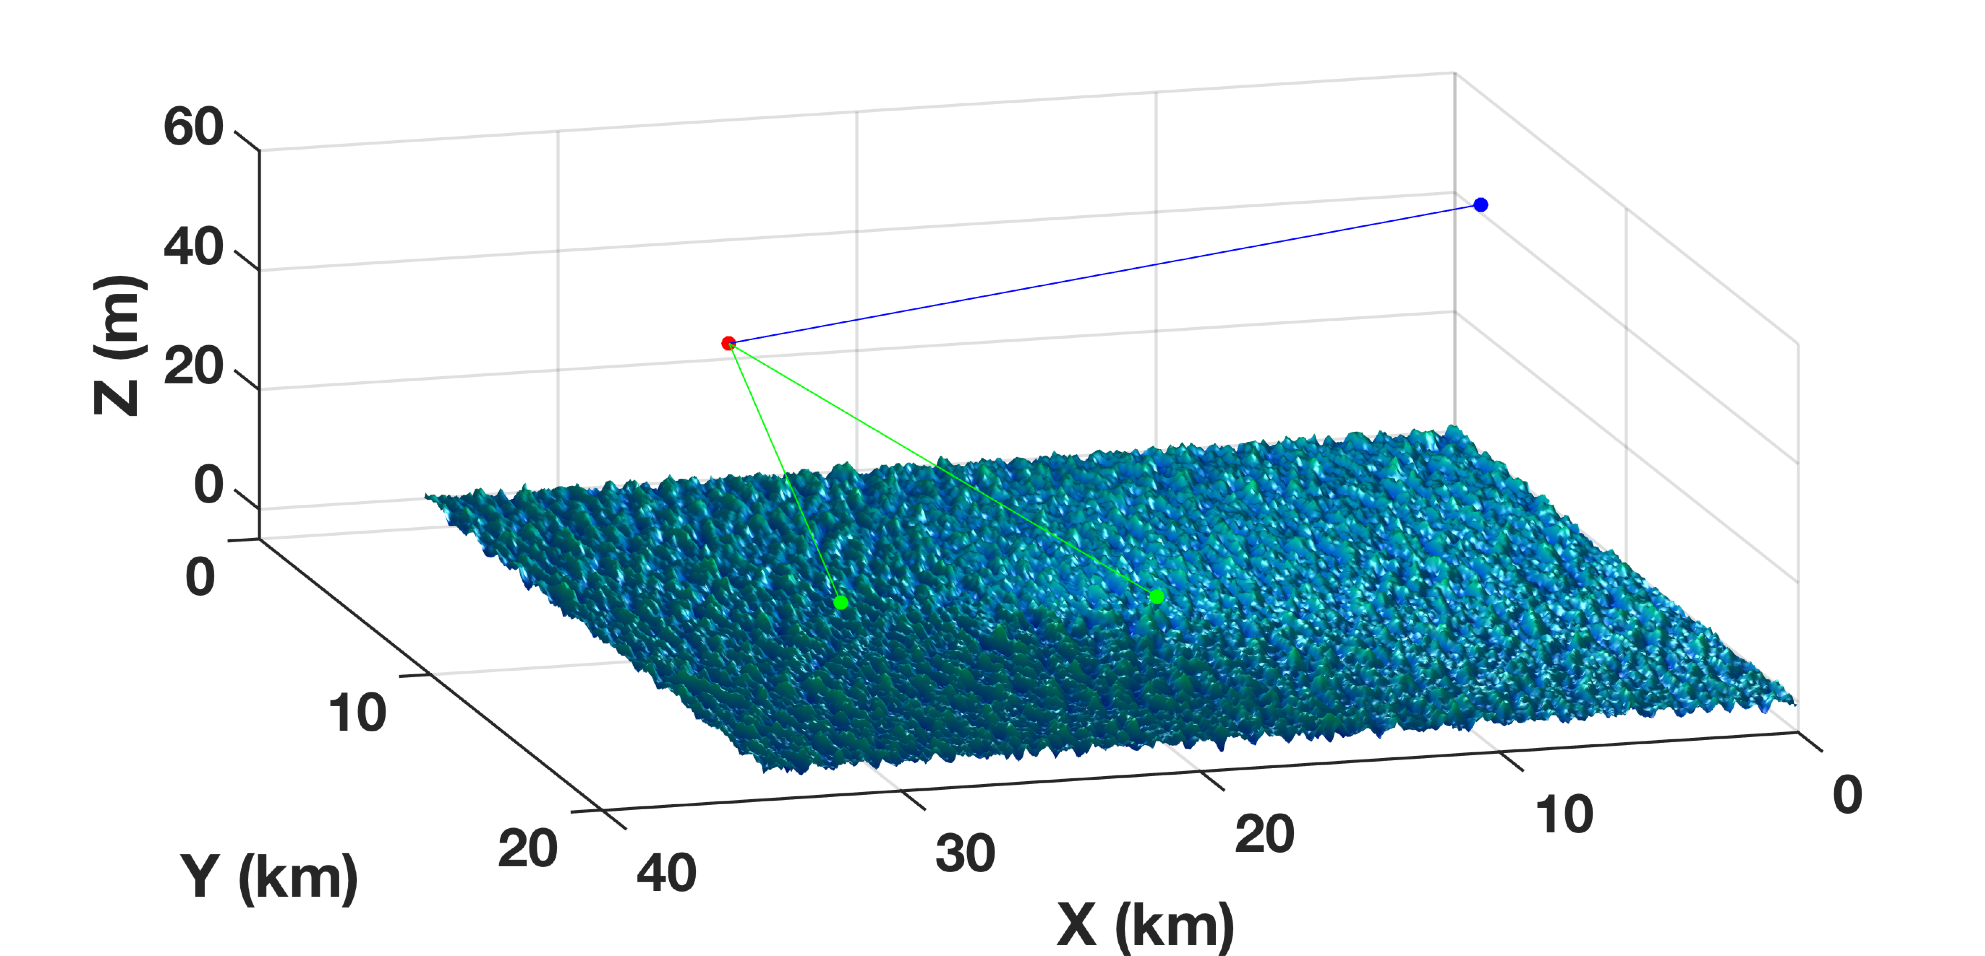
\includegraphics[width=5in]{../media/multistatic/ms_rf_concept2.png}
  \end{center}
  \renewcommand{\baselinestretch}{1} \small\normalsize
  \begin{quote}
    \caption[Example Multi-static Propagation Geometry]{Example Multi-static Propagation Geometry\label{np_fig:1}}
  \end{quote}
\end{figure}
\renewcommand{\baselinestretch}{2} \small\normalsize

Because the receiver and transmitter are not colocated, we cannot leverage reciprocity for the primary path and will need to propagate along both paths. We can however keep the propagation domain to 1-dimension. This is accomplished by generating a sea surface with the wind direction relative to the line of sight between the transmitter and the target for the first path and relative to the line of sight between the receiver and the target for the second path.